\documentclass[]{beamer}
% \geometry{papersize={16cm,9.60cm}}
\usepackage{etex}
\usepackage{amsmath}
\usepackage{tikz}
\usepackage{multimedia}
\usetheme{Boadilla}
\usepackage{graphicx}
%\usepackage{inputenc}

% \mode<presentation>
% {
%   \usetheme{default}
%   \setbeamercovered{transparent}
% }


% {\vskip5pt}

%% customize layout, bullet points navigation toolbar
\setbeamertemplate{navigation symbols}{}%remove navigation symbols
\setbeamertemplate{enumerate items}[default]
\setbeamertemplate{navigation symbols}{}
\setbeamertemplate{itemize items}[circle]
\setbeamercolor{enumerate item}{fg=black}

\setbeamertemplate{footline}{}
\setbeamersize{text margin left = 2.0em}
\setbeamersize{text margin right = 2.0em}

\usepackage{times}
\usepackage[T1]{fontenc}

% Or whatever. Note that the encoding and the font should match. If T1
% does not look nice, try deleting the line with the fontenc.

\setbeamertemplate{navigation symbols}{}

\title{ Cognitive (Neuro) Psychology }
\subtitle{VI. Scaling Methods}
\author{ Marianne Maertens }
\institute[TU Berlin]{Technische Universit\"at Berlin}
\date{July 2016}

\begin{document}
\setbeamertemplate{enumerate items}[default]
\setbeamertemplate{headline}

\frame{\titlepage}

\AtBeginSection[]
{
  \begin{frame}<beamer>
    \frametitle{Layout}
    \tableofcontents[currentsection]
  \end{frame}
}

\begin{frame}
 \frametitle{So far ...}

\end{frame}


\begin{frame}
 \frametitle{Perceptual Scales}
 \begin{itemize}
  \item psychological scales
  \item sensory scales
  \item transducer functions
 \end{itemize}

describe the relationship between the \textcolor{blue}{perceived} and \textcolor{blue}{physical} magnitudes of a stimulus, e.g. transparency and perceived transparency
% \includegraphics[width=50mm]{}
\end{frame}


\begin{frame}
 \frametitle{Types of perceptual scales}
\begin{center}
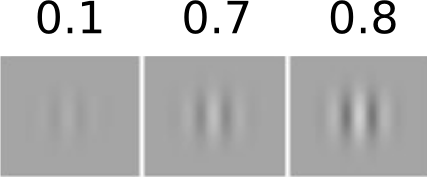
\includegraphics[width=50mm]{figs/l6/three_contrasts.png} 
\end{center}

\textcolor{blue}{ordinal:}
\begin{itemize}
 \item  number stimulus magnitudes according to their rank order along perceptual continuum, difference between any pair of number does not necessarily correspond to magnitude of the perceptual difference, e.g. 1, 2, 3 
 \item differences between numbers do not correspond to perceived differences
\end{itemize}
\end{frame}


\begin{frame}
 \frametitle{Types of perceptual scales}
\begin{center}
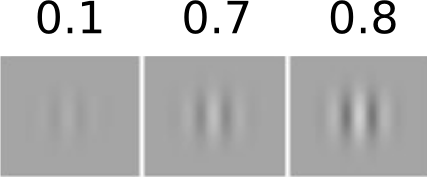
\includegraphics[width=50mm]{figs/l6/three_contrasts.png} 
\end{center}

\textcolor{blue}{interval:}
\begin{itemize}
 \item interval: differences between number correspond to perceptual differences, even though numbers themselves are arbitrary, e.g. 1, 5, 6 or 4, 12, 14, an interval scale can be transformed without loss of information by the equation $aX+b$
 \item does not capture perceived relative magnitudes of the stimulus dimension
\end{itemize}
\end{frame}


\begin{frame}
 \frametitle{Types of perceptual scales}
\begin{center}
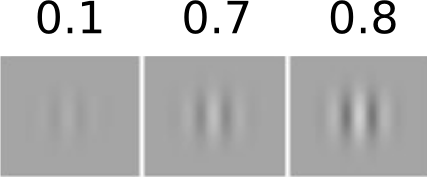
\includegraphics[width=50mm]{figs/l6/three_contrasts.png} 
\end{center}

\textcolor{blue}{ratio:}
\begin{itemize}
 \item interval: capture relative perceived magnitudes, e.g. values of 1 and 5 indicate that the second value is five times the first 
\end{itemize}
\end{frame}


\begin{frame}
 \frametitle{Forced-choice vs. non-forced choice scaling procedures}
\begin{itemize}
 \item
\end{itemize}
\end{frame}

\begin{frame}
 \frametitle{Example: Multi-partition scaling}
\begin{center}
\includegraphics<1>[width=70mm]{figs/l6/whittle_display.png} 
\includegraphics<2>[width=70mm]{figs/l6/whittle_scale.png} 
\end{center}
\end{frame}



\begin{frame}
 \frametitle{General principle of a perceptual scale}
 
\begin{itemize}
 \item perceptual scale is power function $\Psi(x) = a*S^n$
 \item quadruples
 \item equal physical magnitudes, different perceptual magnitudes and vice versa
\end{itemize}

\begin{center}
\includegraphics<1>[width=70mm]{figs/l6/whittle_display.png} 
\end{center}
\end{frame}



\begin{frame}
 \frametitle{Maximum Likelihood Difference Scaling - MLDS \\ \scriptsize{Maloney \& Yang, 2003}}
 
\normalsize
\begin{itemize}
 \item forced-choice scaling procedure
 \item state-of-the-art optimization
 \item produces interval perceptual scale
\end{itemize}
\end{frame}



\begin{frame}
 \frametitle{How MLDS works}
\begin{itemize}
 \item set of stimulus magnitudes $S_1, S_2, S_3, ..., S_n$
 \item $\Psi(2), \Psi(3), \Psi(4), ..., \Psi(n-1)$ are free parameters that have to be estimated, $\Psi(1)$ and $\Psi(n)$ are fixed at 0 and 1
 \item[]
 \item<2-> trial 1: $S_1,S_2$ and $S_3,S_4$, 
 \item<2-> observer: $S_1,S_2$ is more different 
 \item<2-> for a given test set of $\Psi(S)$s MLDS calculates the probability that a hypothetical observer characterized by these parameters will respond that $S_1,S_2$ has the larger perceived difference = likelihood for this trial
 \item[] 
 \item<3-> likelihoods of all trials are multiplied to obtain across-trials likelihood
\end{itemize}
\end{frame}


\begin{frame}
 \frametitle{Single trial example}
\begin{overlayarea}{120mm}{70mm}
\begin{itemize}
 \item initial guesses for parameters:
 \item[] $\Psi(1)=0.5$, $\Psi(2)=0.7$, $\Psi(3)=0.2$, $\Psi(4)=0.3$ 
 \item internal decision noise is: $\sigma_d=0.1$
 \item[]
 \item[$\Rightarrow$] $L(S_1,S_2)|(\Psi(1),\Psi(2),\Psi(3),\Psi(4))$
 \item[]
\end{itemize}
\only<2->{
 $D = |\Psi(2)-\Psi(1)| - |\Psi(4)-\Psi(3)| = |(0.7-0.5)|-|0.3-0.2| = 0.1$
}
\begin{itemize}
\item[] 
\item<3-> convert to z-score $\frac{D}{\sigma_d} = 1$
 \item<3-> calculate area under the standard normal distribution $\Phi(z=1)=0.8413$
\end{itemize}
\end{overlayarea}
\end{frame}



\begin{frame}
 \frametitle{}
\begin{itemize}
 \item
\end{itemize}
\end{frame}


\begin{frame}
 \frametitle{Relationship between z-scores and probabilities}
\begin{center}
\includegraphics<1>[width=50mm]{../../../figures/pmf.png} 
\end{center}

\begin{itemize}
\setlength{\itemsep}{5pt}
 \item subdiscipline of psychology
 \item addresses the relationship between physical stimuli, $x$, and their subjective correlates (percepts), $\Psi(x)$ 
\end{itemize}
\end{frame}


\begin{frame}
 \frametitle{Summary}
\begin{itemize}
 \item 
\end{itemize}
\end{frame}


\begin{frame}
 \frametitle{References}
\begin{small}
\begin{itemize}
 \item  Kingdom \& Prins, Psychophysics. A practical introduction. 
 \item 
 \item 
\end{itemize}
\end{small}
\end{frame}

\end{document}